\section{Equazione del trasporto radiativo}\label{sec:intro-trasporto-radiativo}
Come anticipato nel paragrafo~\ref{sec:astrofisica-osservativa}, per poter interpretare in maniera corrette le misure di radiazione, è necessario studiare i meccanismi di \emph{interazione tra la radiazione e la materia}. Le cause principali di tale interazione sono l'\emph{assorbimento}, lo \emph{scattering}\footnote{deviazione rispetto alla direzione di propagazione originale} e l'\emph{emissione}. Questi fenomeni variano a seconda della \emph{frequenza} e questo è il motivo per cui osservare a frequenze diverse porta a informazioni diverse.

L'\emph{equazione del trasporto radiativo} descrive il trasporto di radiazione da parte dei fotoni. Non è l'unico meccanismo di trasporto ma è il più comune nell'universo. In particolare, l'equazione dice come varia l'intensità della radiazione a causa dell'interazione tra la radiazione e la materia. Prima di ricavare l'equazione è necessario introdurre alcune grandezze indispensabili per indicare le energie.

\subsection{Intensità specifica o brillanza}\label{sec:intensità}
Dato un campo di radiazione, l'intensità specifica $I_\nu$ lungo la direzione $k$, in un punto qualsiasi $P$ del campo, è la quantità di energia che, in un intervallo di tempo $\ud t$ e nell'intervallo di frequenze $\ud \nu$, attraversa una superficie infinitesima perpendicolare alla direzione $k$ ($\ud A_\perp$), entro un angolo solido elementare $\ud \Omega$:
\begin{equation}\label{eq:intensità}
    I_\nu = \frac{\ud E}{\ud t \ud \nu \ud A \ud \Omega \cos{\theta}} \quad \bigl[\si{erg.s^{-1}.cm^{-2}.Hz^{-1}.sr^{-1}}\bigr]
\end{equation}
dove $\theta$ è l'angolo tra la normale a $\ud A$ e la direzione $k$, ovvero posso scrivere: $\ud A_\perp = \ud A \cos{\theta}$. Si guardi la figura~\ref{fig:intensità-specifica}.

\begin{figure}
\centering
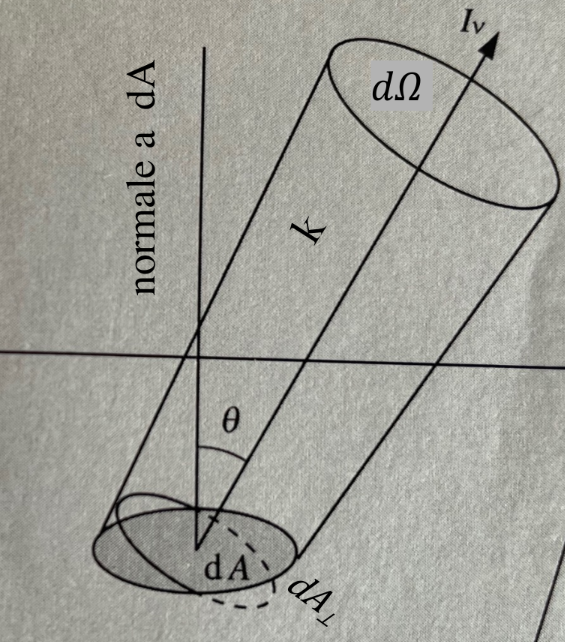
\includegraphics[width=0.3\textwidth]{immagini/intensita-specifica.png}
\caption{Definizione di intensità specifica. $\ud A$ è un'area infinitesima sulla superficie della stella, $P$ è il punto della superficie della stella, $k$ è il versore rispetto al quale definisco l'intensità e $\ud A_\perp = \ud A \cos{\theta}$. La radiazione è portata da un fascio di fotoni, quindi devo considerare un tronco di angolo solido $\ud \Omega$, in cui $\ud A$ rappresenta la sezione del fascio.}
\label{fig:intensità-specifica}
\end{figure}

Si tratta di una proprietà \emph{intrinseca} del campo di radiazione, ovvero della sorgente e si noti come sia definita per unità di frequenza o equivalentemente di lunghezza d'onda.

Si ricordi, inoltre, che il differenziale di angolo solido si scrive:
\begin{equation}\label{eq:angolo-solido}
    \ud \Omega = \sin{\theta} \ud \theta \ud \phi
\end{equation}

Più avanti vedremo uno spettro o \emph{distribuzione spettrale di energia (SED)}. Si tratta della dipendenza dell'intensità dalla lunghezza d'onda (equivalentemente dalla frequenza). 

\subsection{Luminosità}\label{sec:luminosità}
La \emph{luminosità bolometrica} ($L$) di una sorgente è definita come la quantità di energia totale emessa dalla sorgente nell'unità di tempo. Si misura in $\si{erg.s^{-1}}$ oppure in \emph{luminosità solari}, dove $\si{\solarluminosity} = \SI{3.8e33}{erg.s^{-1}}$. Essa è una quantità \emph{intrinseca} della sorgente.

La \emph{luminosità monocromatica} ($L_\nu$) è la luminosità per unità di frequenza (o lunghezza d'onda), cioè la quantità di energia totale emessa dalla sorgente nell'unità di tempo e nell'intervallo di frequenze tra $\nu$ e $\nu + \ud \nu$. $L_\nu$ si misura in $\si{erg.s^{-1}.Hz^{-1}}$, mentre $L_\lambda$ si misura in $\si{erg.s^{-1}.cm^{-1}}$. È semplice ricavare la relazione che lega $L_\nu$ e $L_\lambda$, considerando che $\nu = c / \lambda$. Da questo segue che a un aumento di $\lambda$ corrisponde una diminuzione di $\nu$, ovvero $L_\nu \ud \nu = - L_\lambda \ud \lambda$ e anche che $\ud \nu / \ud \lambda = - c / \lambda^2$. Menttendo le due espressioni insieme si ottiene:
\begin{equation}\label{eq:luminosità-monocromatica}
    L_\lambda = \frac{c}{\lambda^2} L_\nu
\end{equation}

Inoltre è semplice ottenere la luminosità bolometrica a partire da quella monocromatica, è infatti sufficiente integrare su tutte le frequenze:
\begin{equation}\label{eq:luminosità-bolometrica}
    L = \int_0^\infty L_\nu \ud \nu = \int_0^\infty L_\lambda \ud \lambda
\end{equation}
Infatti, per il \emph{teorema di Fourier} è possibile scomporre un'onda nelle sue componenti monocromatiche e nel computo dell'intensità bolometrica considero il contributo di tutte le frequenze.

Ci si può ora chiedere, quale sia la relazione tra l'intensità specifica e la luminosità.

\subsection{Relazione tra intensità e luminosità}\label{sec:relazione-intensità-luminosità}
Consideriamo un campo di radiazione isotropo, per cui $I_\nu$ è uguale per ogni direzione $k$. Questo significa che se considero una superficie infinitesima $\ud A$, la quantità di radiazione entrante e uscente da tale superficie è la stessa per ogni superficie. La luminosità della sorgente è la quantità di radiazione \emph{emessa} dalla sorgente nel tempo $\ud t$, cioè la quantità di radiazione che \emph{esce} dalla sorgente stessa, ovvero la quantità di radiazione che \emph{esce da ciascuna superficie $\ud A$, integrata sulla superficie totale della sorgente}.

Per ottenere la quantità di radiazione che \emph{esce} da ciascuna superficie infinitesima $\ud A$ bisogna integrare sull'angolo solido dell'emisfera \emph{uscente}, ovvero per $\phi \in [0, 2\pi]$ e $\theta \in [0, \pi/2]$. Si faccia riferimento alla figura~\ref{fig:emisfera-uscente}.

\begin{figure}
\centering
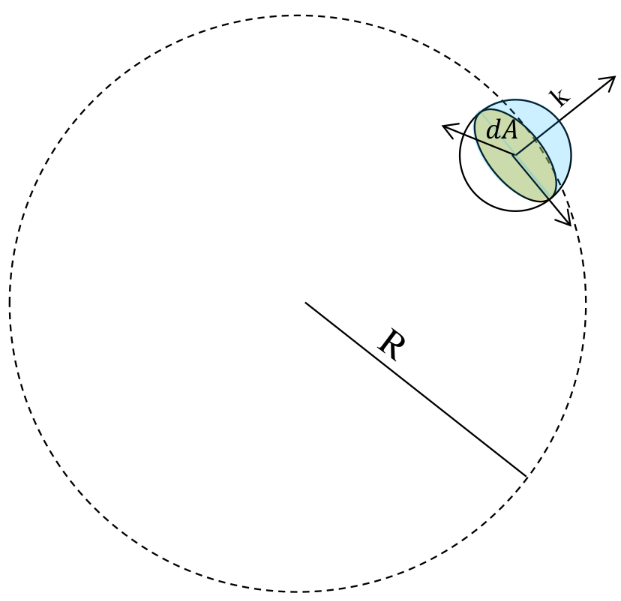
\includegraphics[width=0.3\textwidth]{immagini/emisfera-uscente.png}
\caption{La figura rappresenta un elemento infinitesimo $\ud A$ sulla superficie di una stella. Voglio trovare la radiazione uscente, dunque è quella che attraversa la semisfera uscente che ha come cerchio massimo $\ud A$, poi integro in $\ud A$ per ottenere la radiazione uscente da tutta la superficie della stella}
\label{fig:emisfera-uscente}
\end{figure}

Per ottenere la luminosità totale della sorgente, bisogna integrare su tutta la superficie $4\pi R^2$:
\[
    L_\nu = I_\nu \int_0^{4\pi R^2} \ud A \int_0^{2\pi} \ud \phi \int_0^{\pi/2} \ud \theta \sin{\theta} \cos{\theta}
\]
dove $I_\nu$ è stato portato fuori dal segno di integrale perché non dipende dagli angoli poiché la sorgente è isotropa. Sviluppando i conti si ottiene un'espressione per la luminosità monocromatica
\begin{equation}\label{eq:luminosità-monocromatica-intensità}
    L_\nu = 4 \pi R^2 \pi I_\nu
\end{equation}
e integrando su tutte le frequenze si ottiene la luminosità bolometrica
\begin{equation}\label{eq:luminosità-intensità}
    L = 4 \pi R^2 \pi I
\end{equation}

\subsection{L'equazione e le sue soluzioni}\label{sec:trasporto-radiativo}\label{sec:soluzioni-trasporto-radiativo}

\begin{figure}
\centering
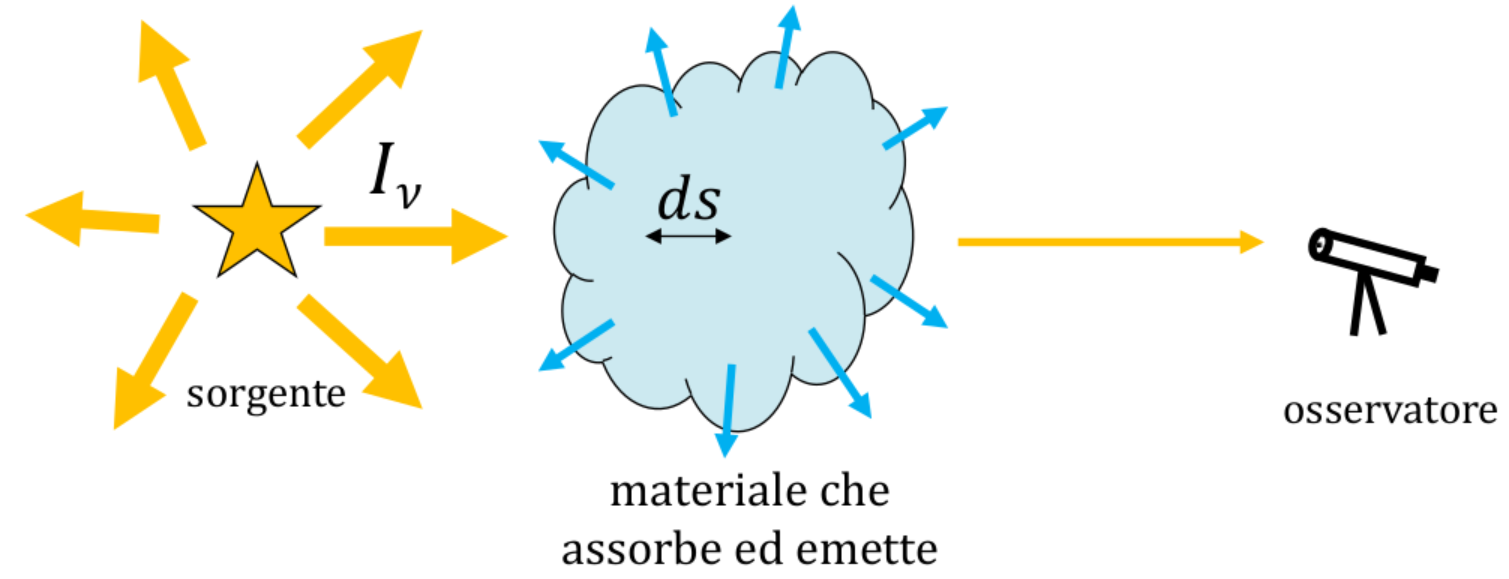
\includegraphics[width=0.7\textwidth]{immagini/trasporto-radiativo.png}
\caption{Equazione del trasporto radiativo. Si studia la variaione di intensità della radiazione emessa dalla sorgente a seguito dell'interazione con il materiale interposto, che avviene attraverso assorbimenti e emissioni. Lo scattering entra nell'assorbimento, poiché l'effetto è quello di deviare la radiazione, e ciò comporta il fatto che misuro una intensità minore di quella iniziale.}
\label{fig:trasporto-radiativo}
\end{figure}

Come già anticipato nel paragrafo~\ref{sec:intro-trasporto-radiativo}, l'\emph{equazione del trasporto radiativo} descrive la variazione dell'intensità della radiazione a causa dell'interazione tra la radiazione stessa e la materia. Infatti, prima di arrivare all'osservatore, la radiazione attraversa della materia, e l'interazione con tale materia provoca assorbimento ed emissione (figura~\ref{fig:trasporto-radiativo}). L'equazione si presenta così:
\begin{equation}\label{eq:trasporto-radiativo}
    \ud I_\lambda = - k_\nu \rho I_\nu \ud S + j_\nu \ud S
\end{equation}
dove appaiono i seguenti termini:
\begin{description}
    \item[$\ud I_\nu$] variazione dell'intensità specifica
    \item[$k_\nu$] coefficiente di assorbimento per unità di massa o opacità ($\si{cm^2.g^{-1}}$). L'opacità ha le dimensioni di una sezione d'urto per unità di massa ed esprime quanta radiazione viene assorbita per unità di massa e per lunghezza attraversata.
    \item[$\rho$] densità di massa del materiale attraversato
    \item[$I_\nu$] intensità in input
    \item[$\ud S$] dimensione infinitesima del materiale attraversato
    \item[$j_\nu$] coefficiente di emissione (\si{erg.s^{-1}.cm^{-3}.Hz^{-1}-sr^{-1}})
\end{description}

In genere si definisce:
\[
\alpha_\nu = k_\nu \rho
\]
e l'equazione assume la seguente forma:
\begin{equation}\label{eq:trasporto-radiativo2}
    \frac{\ud I_\nu}{\ud S} = -\alpha_\nu I_nu + j_\nu
\end{equation}

Si può risolvere l'equazione immediatamente in due casi particolarmente semplici. Nel caso si \emph{pura emissione}, corrispondente a $\alpha_\nu = 0$ si ha:
\[
    \frac{\ud I_\nu}{\ud S} = j_nu \qquad I_\nu = I_\nu (0) + \int \ud S j_\nu
\]
In questo caso l'aumento di densità è pari al coefficiente di emissione integrato lungo la linea di vista.

Nel caso di \emph{puro assorbimento}, corrispondente a $j_\nu = 0$, si ha:
\[
\frac{\ud I_\nu}{\ud S} = -\alpha_\nu I_\nu \quad 
I_\nu (S = I_\nu (0) e^{-\int \alpha_\nu \ud S}
\]
In questo caso l'intensità cala come l'esponenziale del coefficiente di assorbimento intergato lungo la linea di vista.

È conveniente introdurre la \emph{profontià ottica}:
\begin{equation}\label{eq:profondità-ottica}
        \tau_\nu = \int k_\nu \rho \ud S
\end{equation}
dove sto integrando lungo il cammino $\ud S$. La profondità ottica in generale dipende anche dalla frequenza ed è un numero puro. 

È conveniente introdurre anche la \emph{funzione sorgente}:
\begin{equation}\label{eq:funzione-sorgente}
    S_\nu = \frac{j_\nu}{k_\nu \rho} = \frac{j_\nu}{\alpha_\nu}
\end{equation}
Essa esprime il rapporto tra il coefficiente di emissione e quello di assorbimento in termini di $\alpha$ e ha le stesse unità di misura di una intensità specifica.

Con queste due nuove variabili, l'equazione assume una forma particolarmente semplice:
\begin{equation}\label{eq:trasporto-radiativo3}
    \frac{\ud I_\nu}{\ud \tau_\nu} = -I_\nu + S_\nu
\end{equation}
Sviluppando i conti, come mostrato in appendice~\ref{app:trasporto-radiativo} integrando tale equazione si ottiene una soluzione per l'equazione~\eqref{eq:trasporto-radiativo}:
\begin{equation}\label{eq:soluzione-trasporto-radiativo}
    I_\nu = I_{\nu_0} e^{-\tau_\nu} + S_\nu (1- e^{-\tau_\nu})
\end{equation}
Il primo termine è l'intensità iniziale $I_{\nu_0}$(prima dell'interazione con la materia) attenuata da un fattore esponenziale (si ricordi che $\tau \in [1,+\infty]$), mentre il secondo termine \emph{non} dipende dall'intensità iniziale (quella emessa dalla sorgente), ma riguarda solamente il materiale interposto\footnote{Il materiale interposto può anche essere l'atmosfera della stella stessa che si osserva, oppure potrebbe essere l'atmosfera della Terra e così via.}. Trascurando il primo termine, questo secondo termine, che rappresenta l'emissione e l'assorbomento, può anche rappresentare una autoemissione e un autoassorbimento nel caso in cui non ci sia una stella "dietro".

\subsection{Trascuro la sorgente di background}\label{sec:trascuro-sorgente-trasporto-radiativo}
Se nell'equazione~\eqref{eq:soluzione-trasporto-radiativo} trascuro la sorgente di background, assume la forma:
\begin{equation}\label{eq:soluzione-no-sorgente-trasporto-radiativo}
    I_\nu = S_\nu (1- e^{-\tau_\nu})
\end{equation}
Questo corrisponde, ad esempio, a osservare il mezzo interposto da una direzione perpendicolare rispetto alla stella, come mostrato in figura~\ref{fig:trasporto-radiativo-perpendicolare}. Il primo termine, $S_\nu$ rappresenta l'emissione, mentre il secondo termine, $S_\nu e^{-\tau_\nu}$ rappresenta l'auto-assorbimento. Si può studiare questo caso considerando due situazioni limite:
\begin{description}
    \item[Regime otticamente spesso] la profondità ottica è molto grande, $\tau_\nu \gg 1$ , quindi l'intensità coincide con la funzione sorgente: $I_\nu = S_\nu$
    \item[Regime otticamente sottile] la profondità ottica è molto piccola, $\tau_\nu \ll 1$, quindi l'intensità risulta: $I_\nu = S_\nu \tau_\nu$
\end{description}

\begin{figure}
\centering
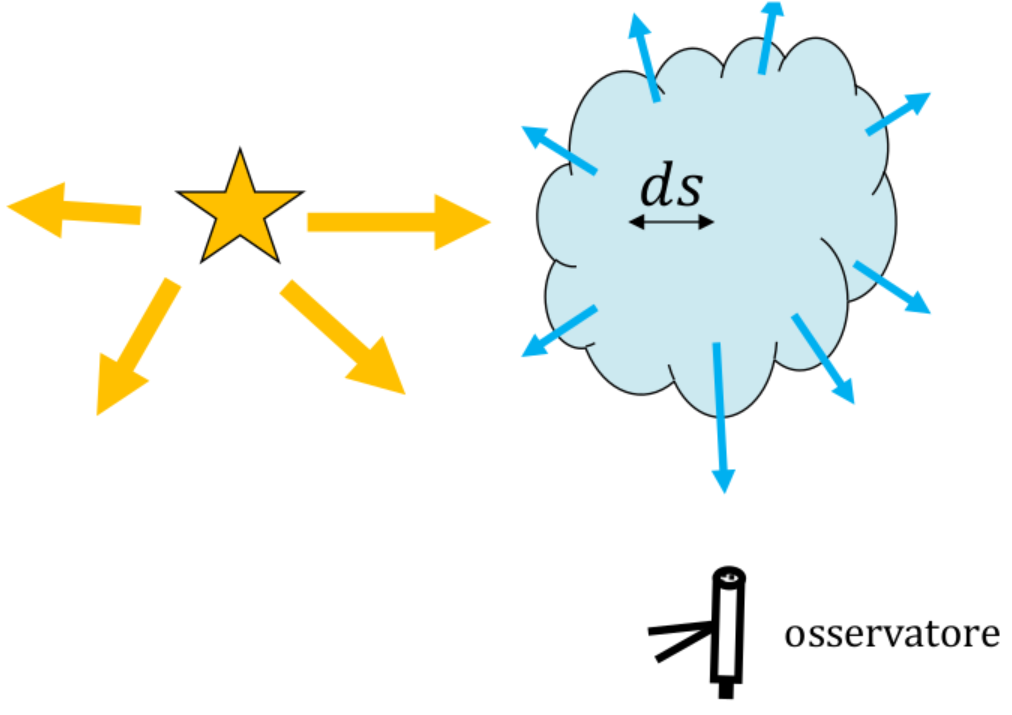
\includegraphics[width=0.4\textwidth]{immagini/trasporto-radiativo-perpendicolare.png}
\caption{Trascuro la sorgente di background nella soluzione dell'equazione del trasporto radiativo.}
\label{fig:trasporto-radiativo-perpendicolare}
\end{figure}

Ci si può chiedere come sia fatta la funzione sorgente $S_\nu$, definita tramite eq.~\eqref{eq:funzione-sorgente}. Essa è diversa a seconda del tipo di radiazione, cioè del processo responsabile del fenomeno di radiazione che sto osservando. Tipicamente i processi di emissione vengono raggruppati in processi termici e processi non termici.
\begin{description}
    \item[Radiazione termica] emessa da un corpo in equilibrio termico (o termodinamico). Ovvero materia e radiazione sono accoppiate, ci sono continui processi di emissione e assorbimento di fotoni e il tasso di assorbimento è uguale al tasso di emissione. Esempi di processi termici sono:
    \begin{itemize}
        \item Radiazione di corpo nero (stelle)
        \item Bremsstrahlung (gas negli ammassi di galassie)
    \end{itemize}
    
    \item[Radiazione non termica] non sono dovuti a processi di emissione e assorbimento, ma, ad esempio, da moto di cariche elettriche oppure da scattering. Esempio sono:
    \begin{itemize}
        \item Sincrotrone (pulsar)
        \item Compton (effetto Sinyaev-Zel'dovich)
    \end{itemize}
\end{description}

\subsection{Radiazione termica}
Se, nell'approssimazione del paragrafo~\ref{sec:trascuro-sorgente-trasporto-radiativo} considero solamente processi termici, ovvero processi dovuti a continue emissioni e assorbimenti, la funzione sorgente coincide con la \emph{funzione di Planck} (eq.~\eqref{eq:corpo-nero}), che verrà introdotta nel prossimo paragrafo.
\[
    S_\nu = B_{BB} (T)
\]
In questo caso, i due regimi di approssimazione si riducono alle seguenti espressioni:
\begin{description}
    \item[regime otticamente spesso ($\tau_\nu \gg 1$)] $I_\nu = B_{BB}$
    \item[regime otticamente sottile ($\tau_\nu \ll 1$)] $I_\nu = B_{BB} \tau_\nu$
\end{description}
È evidente che, se il regime è \emph{otticamente spesso}, la radiazione termica è \emph{radiazione di corpo nero}.
